\chapter{Comparison of Methods}



\section{Testing Setup}

This section outlines the framework used to evaluate the performance of the proposed UAV navigation methods. The evaluation focuses on three primary metrics: accuracy, runtime, and robustness. These metrics are critical to ensure that the navigation system can reliably operate under diverse and challenging conditions, reflecting real-world scenarios where the UAV may encounter varying environmental factors.

\subsection{Datasets}
Five distinct datasets were selected to rigorously test the methods' generalization and performance across different environments. These datasets were captured using Google Earth at constant altitudes within each dataset, ranging from 5.5 to 6.5 km across datasets. The frames had an average radial movement of approximately 600 pixels between them, with a fixed resolution of 1920x972. This setup ensured that the inference task remained challenging but within practical limitations. In real-world scenarios, the higher frame rate and altitude would result in a greater number of images, which would increase overlap and improve inference accuracy. The datasets used for testing are as follows:

\begin{itemize}
    \item \textbf{CITY1 and CITY2} (Cape Town): Both datasets originate from Cape Town. CITY1 incorporates both rotational and translational changes between frames, while CITY2 includes only translational changes. This distinction allows for the isolation of performance under rotational loads.
    \item \textbf{ROCKY}: Represents rugged terrain with varied features, testing the methods' ability to handle complex topographies.
    \item \textbf{DESERT and AMAZON}: Characterized by extreme sparsity and repetitive patterns, these datasets present significant challenges even for human observers to distinguish differences.
\end{itemize}


\subsection{Testing Structure}

Each method, including feature extraction, local feature matching, rotational estimation, image similarity computation, translational estimation, and optimization techniques, is subjected to rigorous testing based on the following criteria:

\begin{itemize}
    \item \textbf{Accuracy}: Evaluated using the Root Mean Square Error (RMSE) of GPS estimations, accuracy assessments focus on the end error. This is justified because outputs—whether images or degrees—propagate through the pipeline, meaning any errors or poor choices are ultimately reflected in the final GPS error.
    \item \textbf{Accuracy}: Evaluated using the Root Mean Square Error (RMSE) of GPS estimations, accuracy assessments focus on the end error. This approach is preferable because intermediate outputs do not always provide clear indicators of quality. For instance, the number of keypoints can be misleading; without context, it's difficult to determine if they represent good features or excessive noise. Outputs propagate through the pipeline, meaning any errors or poor choices are ultimately reflected in the final GPS error, making it more effective to measure accuracy at the end.
    \item \textbf{Runtime}: The entire system runtime per dataset is assessed to evaluate the computational efficiency of each method. Efficient runtimes are crucial for real-time UAV applications, as delays—combined with pilot and UAV response times—can result in consistently missing the target and failing to follow the intended path. As before, runtime may propagate through the system, and therefore the runtime per line is not necessarily indicative of better performance; Runtime per line is not tested. 
    \item \textbf{Robustness}: Tested to verify each method's stability under parameter variations and challenging conditions. Robust methods maintain consistent performance despite environmental or parameter changes, ensuring reliable UAV navigation across different scenarios.
\end{itemize}

This structured testing approach ensures that each component of the UAV navigation system is thoroughly evaluated, facilitating the selection of methods that deliver optimal performance across all critical metrics.

\subsection{Parameters}  
Parameters were held constant across tests and chosen to ensure optimal performance across methods. The focus was not on selecting the absolute best parameter set, as this was not relevant for inter-method testing; rather, the goal was to minimize bias while allowing each method to perform effectively. For instance, multiple methods were tested within a single runtime to enhance testing speed without compromising the integrity of the inter-method comparisons. The takeaway here is to avoid interpreting results objectively, as they do not reflect the realistic and overall performance of the system.



\section{Feature Detectors}

This section presents the evaluation results of three feature detectors: ORB, AKAZE, and SuperPoint with LightGlue. The primary objective of this evaluation is to identify the most suitable detector for a UAV navigation system tasked with estimating rotational and translational transformations. Key performance metrics, including RMSE (Root Mean Square Error), runtime, and robustness across multiple datasets, were considered to assess each detector's effectiveness and suitability.


The evaluation focused on three main criteria:
\begin{itemize}
    \item \textbf{Accuracy (RMSE in GPS)}: Measures the precision of transformation estimates.
    \item \textbf{Runtime}: Assesses the computational efficiency of each detector.
    \item \textbf{Robustness}: Evaluates consistency and reliability across different datasets.
\end{itemize}

The results from these tests informed the selection of the most appropriate detector and threshold parameters for the four defined stages utilizing the detected keypoints: rotational alignment for global matching, global similarity computation, precise translation estimation, and precise rotational estimation.

\subsection{Translation Estimation Performance}

Table \ref{tab:rmse_detectors} presents the RMSE values in meters for each feature detector applied to the precise translation estimation stage. AKAZE, utilizing dynamic keypoint targeting, demonstrated the highest accuracy across all datasets while maintaining reasonable runtime. ORB exhibited respectable accuracy but was consistently outperformed by AKAZE. SuperPoint recorded the highest RMSE values, particularly in challenging datasets such as ROCKY and AMAZON, indicating its limited generalizability across diverse environments.

\begin{table}[H]
    \centering
    \caption{RMSE for Various Local Detectors (in meters)}
    \label{tab:rmse_detectors}
    \begin{tabular}{|c|c|c|c|c|c|}
    \hline
    \textbf{Method} & \textbf{CITY1} & \textbf{CITY2} & \textbf{ROCKY} & \textbf{DESERT} & \textbf{AMAZON} \\ \hline
    ORB & 70.89 & 10.56 & 43.32 & 80.66 & 46.39 \\ \hline
    \makecell{\textbf{Dynamic AKAZE} \\ \textbf{(3000 keypoints)}} & 66.80 & 6.91 & 22.48 & 33.07 & 39.27 \\ \hline
    SuperPoint & 72.66 & 15.80 & 114.93 & 31.60 & 329.19 \\ \hline
    \end{tabular}
\end{table}

\subsubsection*{Runtime and Efficiency}

Table \ref{tab:runtime_detectors} illustrates the runtime (in seconds) for each feature detector across different datasets. ORB proved to be the most efficient detector, making it suitable for applications requiring fast processing. Dynamic AKAZE, while exhibiting longer runtimes, achieved a balance between efficiency and accuracy. SuperPoint demonstrated the longest runtimes across all datasets, highlighting its limited applicability for time-sensitive applications unless optimized with GPU acceleration.

\begin{table}[H]
    \centering
    \caption{Runtime for Various Local Detectors (in seconds)}
    \label{tab:runtime_detectors}
    \begin{tabular}{|c|c|c|c|c|c|}
    \hline
    \textbf{Method} & \textbf{CITY1} & \textbf{CITY2} & \textbf{ROCKY} & \textbf{DESERT} & \textbf{AMAZON} \\ \hline
    ORB & 75.25 & 70.77 & 111.64 & 58.29 & 75.34 \\ \hline
    \makecell{\textbf{Dynamic AKAZE} \\ \textbf{(3000 keypoints)}} & 112.18 & 104.16 & 127.86 & 108.86 & 119.76 \\ \hline
    SuperPoint & 338.21 & 292.11 & 307.93 & 277.73 & 291.01 \\ \hline
    \end{tabular}
\end{table}

\subsubsection*{Robustness}

In terms of robustness, AKAZE exhibited the highest consistency in accuracy across different datasets. ORB also performed well but showed greater variability in accuracy across datasets compared to AKAZE. SuperPoint, however, demonstrated significant performance variability, indicating lower robustness across diverse environments.

\subsection{Rotation Estimation Performance}

Table \ref{tab:rmse_rot_comparison} presents the RMSE values in meters for ORB and AKAZE applied to the precise rotational estimation stage. Both detectors were optimized for this stage to ensure high accuracy while maintaining reasonable runtime.

\begin{table}[H]
    \centering
    \caption{RMSE for ORB (8000 keypoints) and AKAZE (6000 keypoints) (in meters)}
    \label{tab:rmse_rot_comparison}
    \begin{tabular}{|c|c|c|c|c|c|}
    \hline
    \textbf{Method} & \textbf{CITY1} & \textbf{CITY2} & \textbf{ROCKY} & \textbf{DESERT} & \textbf{AMAZON} \\ \hline
    ORB (8000 keypoints) & 69.42 & 8.17 & 22.38 & 32.55 & 37.93 \\ \hline
    \makecell{\textbf{Dynamic AKAZE} \\ \textbf{(6000 keypoints)}} & 68.14 & 8.34 & 21.72 & 35.17 & 39.25 \\ \hline
    \end{tabular}
\end{table}

\subsubsection*{Runtime and Efficiency}

Table \ref{tab:runtime_comparison_rot} presents the runtime comparisons for ORB and AKAZE in the rotational estimation stage. ORB outperformed AKAZE in terms of speed, especially in denser datasets, while maintaining similar levels of accuracy. This suggests that ORB is better suited for time-sensitive applications within this stage.

\begin{table}[H]
    \centering
    \caption{Runtime for ORB (8000 keypoints) and AKAZE (6000 keypoints) (in seconds)}
    \label{tab:runtime_comparison_rot}
    \begin{tabular}{|c|c|c|c|c|c|}
    \hline
    \textbf{Method} & \textbf{CITY1} & \textbf{CITY2} & \textbf{ROCKY} & \textbf{DESERT} & \textbf{AMAZON} \\ \hline
    ORB (8000 keypoints) & 95.80 & 106.63 & 104.79 & 99.56 & 84.70 \\ \hline
    \makecell{\textbf{Dynamic AKAZE} \\ \textbf{(6000 keypoints)}} & 108.44 & 131.10 & 120.77 & 111.25 & 98.70 \\ \hline
    \end{tabular}
\end{table}

\subsubsection*{Robustness}

Regarding robustness, AKAZE demonstrated more consistent accuracy across various datasets compared to ORB, which exhibited greater variability in performance. Despite this, ORB's consistently lower runtimes make it a favorable option for applications where speed is critical.

\subsection{Final Selection of Feature Detectors}

Based on the comprehensive evaluation, the following detectors were selected for the respective stages of the UAV navigation system:

\begin{itemize}
    \item \textbf{Translation Estimation Stage:} 
    AKAZE, with dynamic keypoint targeting (3000 keypoints), exhibited the highest accuracy and robustness in translation estimation while maintaining reasonable runtime. This balance makes Dynamic AKAZE the optimal choice for precise translation inference.
    
    \item \textbf{Rotational Alignment for Translation Estimation Stage:} 
    ORB, utilizing 8000 keypoints, offers an excellent balance between accuracy and efficiency. Although AKAZE demonstrated slightly better performance in rotational estimation, ORB's significantly lower runtime makes it the preferred option for this stage.
    
    \item \textbf{Rotational Alignment for Global Matching Stage:} 
    ORB, with 6000 keypoints, is the optimal choice due to its superior runtime efficiency. This stage can accommodate relatively larger rotational estimation errors, making ORB ideal for global matching tasks.
    
    \item \textbf{Global Similarity Refinement:} 
    ORB, employing 1500 keypoints, is selected for global image similarity comparison using local matching. The lower accuracy requirement and the necessity for high runtime efficiency make ORB the best fit for grid matching.
\end{itemize}

These selections ensure that each stage of the UAV navigation system leverages the most appropriate feature detector, optimizing both accuracy and computational performance.



\section{Local Feature Matchers}

This section evaluates two prominent local matchers, BFMatcher and FLANN, within the context of a UAV navigation system. The primary objective of this evaluation is to determine the most efficient and robust matcher in terms of accuracy, runtime, and consistency across diverse datasets. These matchers play a crucial role in the system's ability to accurately estimate rotational and translational transformations by effectively pairing detected feature points.

\subsection{Testing Overview}

The local matchers were assessed under various conditions to evaluate their performance concerning accuracy (RMSE in GPS), runtime, and robustness. The evaluation was meticulously designed to understand how each matcher handles noisy keypoints, limited post-match filtering, and varying detector thresholds. The goal was to identify which matcher offers the most suitable balance between match quality and computational efficiency, thereby ensuring real-time applicability in UAV navigation.

\subsection{Accuracy Evaluation}

Table \ref{tab:flann_bf_comparison_acc} presents the Root Mean Squared Error (RMSE) in GPS values for BFMatcher and FLANN across different datasets. The results indicate that while BFMatcher achieves slightly better accuracy in certain cases, FLANN remains highly competitive with only marginally higher RMSE values.

\begin{table}[H]
    \centering
    \caption{RMSE GPS Accuracy for BFMatcher and FLANN (in meters)}
    \label{tab:flann_bf_comparison_acc}
    \begin{tabular}{|c|c|c|c|c|c|}
    \hline
    \textbf{Matcher} & \textbf{CITY1} & \textbf{CITY2} & \textbf{ROCKY} & \textbf{DESERT} & \textbf{AMAZON} \\ \hline
    FLANN          & 56.59           & 4.70           & 14.63          & 71.20           & 32.35           \\ \hline
    BFMatcher      & 53.89           & 3.79           & 16.36          & 68.64           & 33.24           \\ \hline
    \end{tabular}
\end{table}

\textbf{Observations:}
\begin{itemize}
    \item \textbf{BFMatcher Accuracy:} BFMatcher demonstrated slightly superior accuracy in CITY1 and CITY2 compared to FLANN. However, the improvement was not substantial enough to outweigh its increased computational demands.
    \item \textbf{FLANN Accuracy:} FLANN maintained competitive accuracy levels, trailing BFMatcher only marginally in most datasets. Notably, FLANN exhibited strong performance in the ROCKY dataset, underscoring its reliability in challenging environments.
\end{itemize}

\subsection{Runtime Evaluation}

Table \ref{tab:flann_bf_comparison_runtime} illustrates the runtime (in seconds) for BFMatcher and FLANN across different datasets. The results clearly show that FLANN consistently outperforms BFMatcher in terms of speed, with significantly lower execution times across all datasets.

\begin{table}[H]
    \centering
    \caption{Runtime Comparison for BFMatcher and FLANN (in seconds)}
    \label{tab:flann_bf_comparison_runtime}
    \begin{tabular}{|c|c|c|c|c|c|}
    \hline
    \textbf{Matcher} & \textbf{CITY1} & \textbf{CITY2} & \textbf{ROCKY} & \textbf{DESERT} & \textbf{AMAZON} \\ \hline
    FLANN          & 42.72           & 41.61          & 41.96          & 43.42           & 53.62           \\ \hline
    BFMatcher      & 203.49          & 228.59         & 46.33          & 52.59           & 88.95           \\ \hline
    \end{tabular}
\end{table}

\textbf{Observations:}
\begin{itemize}
    \item \textbf{FLANN Efficiency:} FLANN exhibited significantly faster runtimes across all datasets, particularly excelling in CITY1 and CITY2 where it completed tasks in less than a quarter of the time required by BFMatcher.
    \item \textbf{BFMatcher Runtime:} The exhaustive matching approach of BFMatcher resulted in considerably higher runtimes, rendering it less suitable for real-time applications where speed is critical.
\end{itemize}

\subsection{Robustness Under Varying Detector Thresholds}

Figure \ref{fig:divergence_plot} depicts the divergence in RMSE GPS error between FLANN and BFMatcher as the number of keypoints increases. Positive values indicate that BFMatcher outperforms FLANN, while negative values suggest FLANN performs better.

\begin{figure}[H]
    \centering
    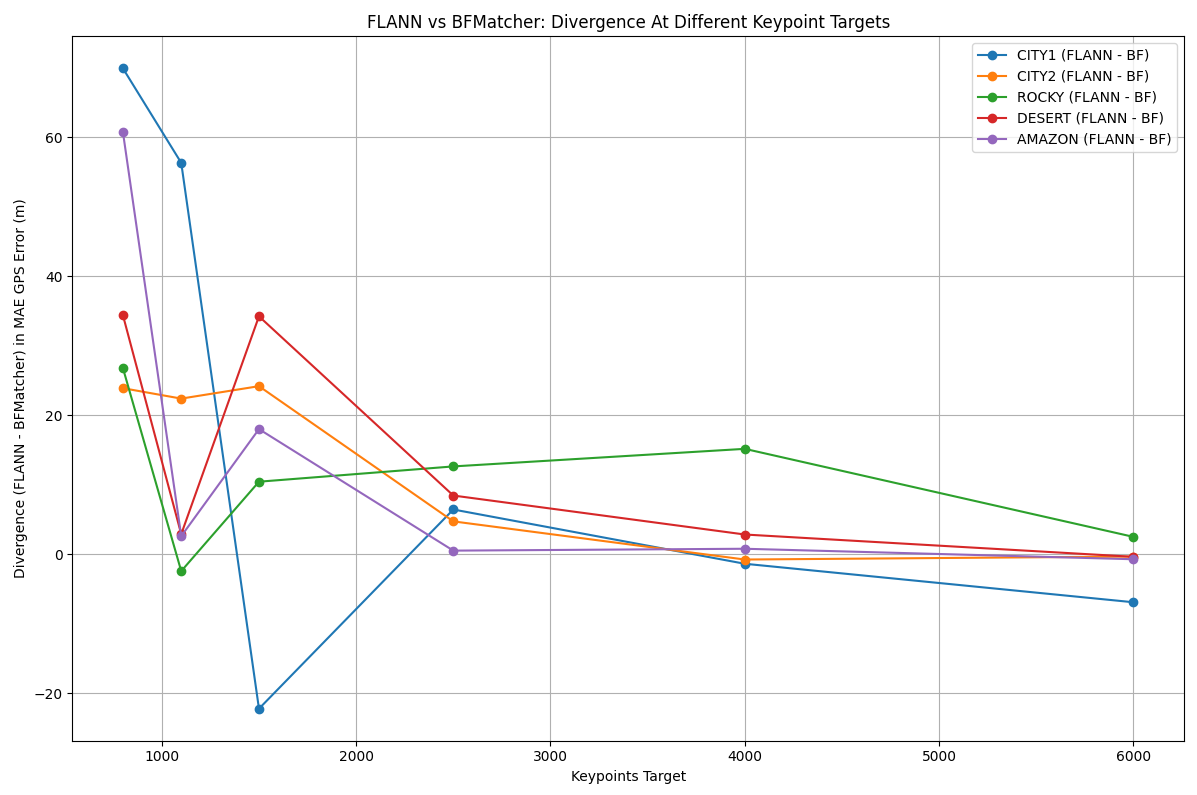
\includegraphics[width=\textwidth]{./Graphs/Divergence_BF_FLANN_KPS.png}
    \caption{Divergence in RMSE GPS Error Between FLANN and BFMatcher Across Keypoint Targets}
    \label{fig:divergence_plot}
\end{figure}

\textbf{Observations:}
\begin{itemize}
    \item \textbf{Convergence:} Both matchers demonstrated similar accuracy levels as the number of keypoints increased, with performance becoming nearly identical beyond 2500 keypoints. Given that feature detectors are typically configured with a keypoint target of at least 3000, both matchers are expected to perform comparably in standard operational conditions.
    \item \textbf{Outliers:} Although BFMatcher generally outperforms FLANN, there are instances where FLANN achieves better accuracy. This can occur due to FLANN’s approximate matching, which may preserve valid matches that BFMatcher might discard using Lowe’s ratio thresholding.
    \item \textbf{Scalability:} FLANN's runtime scalability with increasing keypoint counts was superior to that of BFMatcher, making FLANN a more scalable solution for larger datasets.
\end{itemize}

\subsection{Final Selection of Local Feature Matcher}

Based on the comprehensive evaluation of accuracy, runtime, and robustness, FLANN emerges as the optimal choice for the UAV navigation system. FLANN offers significantly faster runtimes and better scalability while maintaining comparable accuracy to BFMatcher. This makes FLANN highly suitable for real-time applications where computational efficiency is paramount.

\begin{itemize}
    \item \textbf{Overall Choice:} \textbf{FLANN} is selected as the primary local feature matcher for the UAV navigation system, balancing high performance and efficiency across diverse operational conditions.
\end{itemize}

These selections ensure that the UAV navigation system leverages the most appropriate local matcher, optimizing both accuracy and computational performance to achieve reliable and efficient navigation.


\section{Rotational Estimators}
xxx fix
This section evaluates the performance of four rotational estimation methods: Partial Affine 2D, Affine 2D, Homography, and Rigid Via SVD. The objective is to identify the most suitable method for UAV navigation by comparing accuracy, runtime, and robustness across various datasets. These estimators are critical for accurately determining the rotational transformations required for precise navigation and alignment of UAV imagery.

\subsection{Accuracy Evaluation}

The Rigid transforms, SVD and Partial Affine 2D provided the most accurate and consistent results across datasets. They were subsequently tested in conjunction to see if their benefits could be added. However, the SVD only rigid transform performed marginally better across the datasets. Ultimately, the OpenCV methods using outlier rejection sometimes helped improve the estimate, but their use of static thresholds and increased degrees of freedom rendered them less able to maintain this accuracy across datasets. Table \ref{tab:rmse_comparison_rotestim} summarizes the RMSE values (in meters) for the given methods.

\begin{table}[H] 
    \centering 
    \caption{RMSE Comparison Across Datasets for Different Rotational Estimators} 
    \label{tab:rmse_comparison_rotestim} 
    \begin{tabular}{|c|c|c|c|c|c|} 
        \hline
        \textbf{Method} & \textbf{CITY1} & \textbf{CITY2} & \textbf{ROCKY} & \textbf{DESERT} & \textbf{AMAZON} \\ \hline
        Partial Affine 2D & 70.18 & 7.54 & 27.98 & 44.94 & 46.98 \\ \hline 
        Affine 2D & 81.22 & 7.80 & 22.10 & 43.11 & 52.56 \\ \hline 
        Homography & 76.25 & 7.16 & 24.40 & 48.56 & 48.04 \\ \hline 
        Rigid Affine + SVD & 51.72 & 5.98 & 21.18 & 36.27 & 30.84 \\ \hline 
        \makecell{Rigid SVD} & 51.74 & 6.16 & 19.03 & 36.48 & 31.57 \\ \hline 
    \end{tabular} 
\end{table}

\subsection{Runtime Evaluation}

The runtime results below relate mostly to the degrees of freedom in the method, with the simplest rigid transforms performing the best. The SVD only based method performs the fastest due to its lack of iterative optimization and singular method.
Table \ref{tab:runtime_comparison_rotestim} presents the runtime (in seconds) for each rotational estimator across the five datasets. 

\begin{table}[H] 
    \centering 
    \caption{Runtime Comparison Across Datasets for Different Rotational Estimators} 
    \label{tab:runtime_comparison_rotestim} 
    \begin{tabular}{|c|c|c|c|c|c|} 
        \hline 
        \textbf{Method} & \textbf{CITY1} & \textbf{CITY2} & \textbf{ROCKY} & \textbf{DESERT} & \textbf{AMAZON} \\ \hline
        Partial Affine 2D & 56.76 & 52.20 & 69.44 & 56.40 & 50.34 \\ \hline 
        Affine 2D & 65.27 & 54.55 & 76.16 & 71.52 & 58.16 \\ \hline 
        Homography & 68.79 & 65.11 & 78.92 & 69.97 & 58.27 \\ \hline 
        Rigid Affine + SVD & 90.74 & 77.45 & 81.19 & 90.74 & 94.25 \\ \hline 
        \makecell{Rigid SVD} & 83.33 & 61.47 & 77.94 & 71.27 & 74.77 \\ \hline 
    \end{tabular} 
\end{table}
    
    

\subsection{Robustness Testing}

Robustness testing assessed each method's sensitivity to parameter variations, including Lowe’s ratio, RANSAC thresholds, and keypoint quantity. The generalization to datasets was spoken to in accuracy testing. This evaluation was essential to determine the performance consistency of each method under different challenging conditions. For the sake of brevity, the results are omitted; The recorded observations are summarized below.


\textbf{Observations:}  
\begin{itemize}
    \item \textbf{Parameter Sensitivity:} All methods were excellent at being robust against parameter variations, maintaining consistent performance across different settings.
    \item \textbf{Best Robustness:} The Rigid via SVD only transform exhibited the highest robustness across all parameters, especially at low keypoint counts, maintaining consistent performance under varying conditions.

\end{itemize}

\subsection{Final Selection of Rotational Estimator}

Based on the comprehensive evaluation of accuracy, runtime, and robustness, the rigid transform by SVD only emerged as the most suitable rotational estimator for the UAV navigation system. It demonstrated the lowest combined normalized RMSE across all datasets, the fastest runtime, and high robustness. 

\section{Image Similarity Estimators}

Accurate image similarity estimation, or global matching, is essential for UAV navigation systems to choose reasonable images to compare to. They should ensure accuracy and efficiency while maintaining robustness against small rotational offsets. This section evaluates different global matching techniques across multiple datasets to identify the most suitable method for UAV navigation based on accuracy, runtime, and robustness.

\subsection{Accuracy Evaluation}

Naturally, the appropriateness of the choice of best match is implicitly passed through to subsequent stages and realized as an error in GPS estimations. Root Mean Square Error (RMSE) was utilized to assess the GPS estimation accuracy of each global matching technique across the five datasets. Table \ref{tab:RMSE_GLOBAL_MATCHING} summarizes the RMSE values (in meters) for Local Retrofit, Cross Correlation, Histogram, and SSIM.

\begin{table}[H]
    \centering
    \caption{RMSE Comparison Across Datasets for Various Global Matching Techniques (in meters)}
    \label{tab:RMSE_GLOBAL_MATCHING}
    \begin{tabular}{|c|c|c|c|c|c|}
    \hline
    \makecell{Global Matching \\ Technique} & \makecell{CITY1} & \makecell{CITY2} & \makecell{ROCKY} & \makecell{DESERT} & \makecell{AMAZON} \\ \hline
    \makecell{Local Retrofit} & 46.56 & 7.37 & 17.32 & 128.43 & 34.54 \\ \hline
    \makecell{Cross Correlation} & 49.88 & 5.12 & 15.77 & 26.84 & 31.50 \\ \hline
    Histogram & 46.35 & 5.12 & 15.77 & 27.28 & 31.50 \\ \hline
    SSIM & 50.03 & 6.16 & 15.77 & 27.28 & 31.44 \\ \hline
    \end{tabular}
\end{table}

\textbf{Observations:}  
\begin{itemize}
    \item \textbf{Histogram Accuracy:} The Histogram technique consistently achieved the lowest RMSE across most datasets, particularly excelling in CITY1, CITY2, and ROCKY.
    \item \textbf{Cross Correlation Accuracy:} Cross Correlation closely followed Histogram in accuracy, demonstrating strong performance in CITY2 and DESERT.
    \item \textbf{SSIM Accuracy:} SSIM maintained comparable accuracy to Histogram and Cross Correlation but exhibited slightly higher errors in CITY1 and DESERT.
    \item \textbf{Local Retrofit Accuracy:} The Local Retrofit method recorded the highest RMSE values, especially in the DESERT dataset, indicating poor generalizability and higher complexity. Consequently, it was excluded from further analysis.
\end{itemize}

\subsection{Runtime Evaluation}

Table \ref{tab:RUNTIME_GLOBAL_MATCHING} compares the computational efficiency of each global matching technique across the five datasets.

\begin{table}[H]
    \centering
    \caption{Runtime Comparison Across Global Matching Techniques (in seconds)}
    \label{tab:RUNTIME_GLOBAL_MATCHING}
    \begin{tabular}{|c|c|c|c|c|c|}
    \hline
    \makecell{Global Matching \\ Technique} & \makecell{CITY1} & \makecell{CITY2} & \makecell{ROCKY} & \makecell{DESERT} & \makecell{AMAZON} \\ \hline
    \makecell{Local Retrofit} & 84.56 & 76.34 & 70.22 & 63.47 & 90.69 \\ \hline
    \makecell{Cross Correlation} & 59.62 & 56.67 & 54.14 & 59.90 & 65.92 \\ \hline
    Histogram & 57.06 & 56.33 & 56.68 & 51.98 & 59.09 \\ \hline
    SSIM & 91.60 & 77.99 & 83.31 & 83.08 & 114.07 \\ \hline
    \end{tabular}
\end{table}

\textbf{Observations:}  
\begin{itemize}
    \item \textbf{Histogram Efficiency:} The Histogram technique was the most efficient in terms of runtime, outperforming all other methods consistently across all datasets.
    \item \textbf{Cross Correlation Efficiency:} Cross Correlation followed closely behind Histogram, offering slightly higher runtimes but still maintaining high computational efficiency.
    \item \textbf{SSIM Efficiency:} SSIM exhibited the longest runtimes, particularly in the AMAZON and DESERT datasets, rendering it less suitable for real-time applications.
    \item \textbf{Local Retrofit Efficiency:} The Local Retrofit method had the highest runtimes and was deemed non-viable due to its excessive computational cost and poor accuracy.
\end{itemize}

\subsection{Robustness to Rotational Offsets}

Robustness testing evaluated each global matching technique's sensitivity to a 10-degree rotational offset. All matchers that made it this far saw no change in choice combination below a 5-degree offset. The impact on RMSE GPS error and the percentage change in error were recorded to assess each method's stability under rotational misalignments.

\begin{table}[H]
    \centering
    \caption{RMSE (GPS Error) and Percentage Change with 10-degree Rotational Offset}
    \label{Robustness_GlobalMatchers}
    \begin{tabular}{|c|c|c|c|c|c|c|}
    \hline
    \textbf{Method} & \textbf{Metric} & \textbf{CITY1} & \textbf{CITY2} & \textbf{ROCKY} & \textbf{DESERT} & \textbf{AMAZON} \\ \hline
    \multirow{2}{*}{\makecell{Cross Correlation}} & RMSE & 54.81 & 5.34 & 17.55 & 32.51 & 31.52 \\ \cline{2-7}
    & \% Change & 5.89\% & 4.29\% & 11.54\% & 21.92\% & 0.06\% \\ \hline
    \multirow{2}{*}{\makecell{Histogram}} & RMSE & 56.17 & 4.45 & 16.83 & 37.20 & 36.35 \\ \cline{2-7}
    & \% Change & 20.93\% & -13.09\% & 6.73\% & 36.73\% & 15.38\% \\ \hline
    \multirow{2}{*}{\makecell{SSIM}} & RMSE & 55.93 & 5.53 & 16.25 & 41.01 & 31.67 \\ \cline{2-7}
    & \% Change & 11.79\% & -10.23\% & 3.04\% & 50.43\% & 0.73\% \\ \hline
    \end{tabular}
\end{table}

\textbf{Observations:}  
\begin{itemize}
    \item \textbf{Cross Correlation Robustness:} Cross Correlation exhibited the lowest percentage change in GPS error under a 10-degree rotational offset, indicating strong robustness.
    \item \textbf{Histogram Robustness:} While Histogram demonstrated competitive RMSE values, it showed significant deviations in the DESERT and AMAZON datasets when subjected to rotational offsets.
    \item \textbf{SSIM Robustness:} SSIM displayed higher error rates and greater variability, particularly in the DESERT dataset, making it less robust to significant rotational misalignments.
\end{itemize}

\subsection{Improvement Technique}

An additional method, the rigid transform using Singular Value Decomposition (SVD), was initially evaluated as a primary global matching technique. However, it performed significantly worse than the other methods and was subsequently excluded from standalone consideration. However, when the rigid transform was applied after other estimation methods, it consistently enhanced overall accuracy. This improvement is likely due to the rigid transform's ability to make minor, precise corrections once the point cloud is largely aligned by other methods, despite its initial inefficiency in handling large misalignments.

\subsection{Final Selection of Global Matching Technique}

Based on the comprehensive evaluation of accuracy, runtime, and robustness, the \textbf{Histogram} technique is identified and chosen as the most suitable global matching method for the system. Histogram consistently provided superior performance in terms of both RMSE and runtime, particularly under large rotational offsets. Although Cross Correlation also demonstrated strong performance, Histogram's marginally better accuracy and runtime efficiency make it the preferred choice.



\section{Translational Estimators}

This section evaluates the performance of various translational estimation methods for UAV navigation. The methods assessed include Phase Correlation, Rigid Transform, Affine Transform with RANSAC, Homography Transform, and Partial Affine 2D. Each method is evaluated based on accuracy, runtime, and robustness across multiple datasets to identify the most effective option for UAV navigation.

\subsection{Accuracy Evaluation}

Root Mean Square Error (RMSE) was utilized to assess the GPS estimation accuracy of each translational estimation method across five datasets. Table \ref{tab:rmse_comparison_transestim} summarizes the RMSE values (in meters) for each method.

\begin{table}[H]
    \centering
    \caption{RMSE GPS Error Comparison Across Datasets for Different Translation Methods}
    \label{tab:rmse_comparison_transestim}
    \begin{tabular}{|c|c|c|c|c|c|}
    \hline
    \textbf{Method} & \textbf{CITY1} & \textbf{CITY2} & \textbf{ROCKY} & \textbf{DESERT} & \textbf{AMAZON} \\ \hline
    \makecell{\textbf{Phase Corr}}        & 1437.85 & 1349.16 & 629.82 & 1263.15 & 1121.81 \\ \hline
    \makecell{\textbf{Rigid Transform}}   & 64.31   & 7.42    & 21.82  & 29.01   & 38.52   \\ \hline
    \makecell{\textbf{Affine Transform}}  & 127.77  & 88.41   & 57.01  & 70.96   & 118.77  \\ \hline
    \makecell{\textbf{Homography}}        & 168.35  & 92.54   & 58.69  & 120.15  & 242.97  \\ \hline
    \makecell{\textbf{Partial Affine 2D}} & 64.11   & 6.34    & 19.07  & 29.94   & 40.08   \\ \hline
    \end{tabular}
\end{table}

\textbf{Observations:}
\begin{itemize} 
    \item \textbf{Partial Affine 2D} achieved the lowest RMSE, establishing it as the most accurate estimator across all datasets. Its superior performance compared to the direct algebraic \textbf{Rigid Transform} is attributed to the utilization of RANSAC for effective outlier rejection.
    \item Both \textbf{Homography} and \textbf{Affine Transform} methods exhibited significantly higher RMSE values than Partial Affine 2D and Rigid Transform. This increase is primarily due to their greater degrees of freedom and inherent complexity.
    \item \textbf{Phase Correlation} recorded the highest RMSE values, indicating lower accuracy relative to the other methods. This reduced performance is likely due to its heightened sensitivity to noise, as it processes the entire image context.
\end{itemize}

\subsection{Runtime Evaluation}

Table \ref{tab:runtime_comparison_transestim} presents the runtime (in seconds) for each translational estimation method across the five datasets.

\begin{table}[H]
    \centering
    \caption{Runtime Comparison Across Datasets for Different Translation Methods (in seconds)}
    \label{tab:runtime_comparison_transestim}
    \begin{tabular}{|c|c|c|c|c|c|}
    \hline
    \textbf{Method} & \textbf{CITY1} & \textbf{CITY2} & \textbf{ROCKY} & \textbf{DESERT} & \textbf{AMAZON} \\ \hline
    \makecell{\textbf{Phase Corr}}        & 1437.85 & 1349.16 & 629.82 & 1263.15 & 1121.81 \\ \hline
    \makecell{\textbf{Rigid Transform}}   & 89.05   & 99.74   & 103.46 & 104.84  & 87.43   \\ \hline
    \makecell{\textbf{Affine Transform}}  & 127.77  & 88.41   & 57.01  & 70.96   & 118.77  \\ \hline
    \makecell{\textbf{Homography}}        & 168.35  & 92.54   & 58.69  & 120.15  & 242.97  \\ \hline
    \makecell{\textbf{Partial Affine 2D}} & 94.62   & 82.77   & 85.94  & 72.43   & 78.33   \\ \hline
    \end{tabular}
\end{table}

\textbf{Observations:}  
\begin{itemize}
    \item \textbf{Partial Affine 2D} demonstrated the fastest runtime among the translational methods, making it the most computationally efficient. It was followed by the \textbf{Rigid Transform}.
    \item \textbf{Phase Correlation} exhibited significantly longer runtimes, making it less viable for real-time UAV applications.
\end{itemize}

\subsection{Robustness Testing}

Robustness was assessed by evaluating each method's sensitivity to parameter variations, such as keypoint quantity and threshold changes. Table \ref{tab:variance_transestim} highlights the standard deviation of RMSE across datasets to indicate consistency.

\begin{table}[H]
    \centering
    \caption{RMSE Variance Across Datasets for Different Translation Methods (Robustness Test)}
    \label{tab:variance_transestim}
    \begin{tabular}{|c|c|c|c|c|c|}
    \hline
    \textbf{Method} & \textbf{CITY1} & \textbf{CITY2} & \textbf{ROCKY} & \textbf{DESERT} & \textbf{AMAZON} \\ \hline
    \makecell{\textbf{Phase Corr}}        & 111.35 & 76.54  & 55.69  & 110.15 & 101.97 \\ \hline
    \makecell{\textbf{Rigid Transform}}   & 64.61  & 7.53   & 21.14  & 31.31  & 37.96  \\ \hline
    \makecell{\textbf{Affine Transform}}  & 127.77 & 88.41  & 57.01  & 70.96  & 118.77 \\ \hline
    \makecell{\textbf{Homography}}        & 168.35 & 92.54  & 58.69  & 120.15 & 242.97 \\ \hline
    \makecell{\textbf{Partial Affine 2D}} & 64.11  & 6.34   & 19.07  & 29.94  & 40.08  \\ \hline
    \end{tabular}
\end{table}

\textbf{Observations:}  
\begin{itemize}
    \item \textbf{Partial Affine 2D} and \textbf{Rigid Transform} exhibited the lowest variance, indicating strong robustness to parameter changes.
    \item \textbf{Homography} showed the most variability and performed inconsistently under different conditions.
\end{itemize}

\subsection{Final Choice of Translational Estimator}

Based on the evaluation of accuracy, runtime, and robustness, \textbf{Partial Affine 2D} was selected as the most suitable translational estimator for the UAV navigation system. It demonstrated the highest accuracy, fastest runtime, and strong robustness across all datasets.

\begin{itemize}
    \item \textbf{Primary Translational Estimator:} \textbf{Partial Affine 2D} is chosen for its optimal performance in minimizing GPS error, computational efficiency, and consistent robustness across diverse operational conditions.
\end{itemize}




\section{Optimization Techniques}

This section outlines the selected optimization methods and their corresponding parameter choices for each stage of the UAV navigation system. The focus is on the robustness of each technique and the comparative performance of different methods, rather than on identifying the absolute optimal parameters for each dataset.

\subsection{Planar Transform Outlier Rejection Method}

Two outlier rejection methods, LMEDS (Least Median of Squares) and RANSAC (Random Sample Consensus), were evaluated for planar transform estimation. The performance comparison is summarized in Tables \ref{tab:rmse_comparison_opt} and \ref{tab:runtime_comparison_opt}.

\begin{table}[H]
    \centering
    \caption{RMSE Comparison Across Datasets for LMEDS and RANSAC}
    \label{tab:rmse_comparison_opt}
    \begin{tabular}{|c|c|c|}
    \hline
    \textbf{Dataset} & \textbf{RMSE GPS Error (LMEDS)} & \textbf{RMSE GPS Error (RANSAC)} \\ \hline
    CITY1   & 51.78 & 59.57 \\ \hline
    CITY2   & 6.16  & 5.84  \\ \hline
    ROCKY   & 19.04 & 18.59 \\ \hline
    DESERT  & 36.48 & 35.90 \\ \hline
    AMAZON  & 31.57 & 34.48 \\ \hline
    \end{tabular}
\end{table}

\begin{table}[H]
    \centering
    \caption{Runtime Comparison Across Datasets for LMEDS and RANSAC}
    \label{tab:runtime_comparison_opt}
    \begin{tabular}{|c|c|c|}
    \hline
    \textbf{Dataset} & \textbf{Runtime (LMEDS)} & \textbf{Runtime (RANSAC)} \\ \hline
    CITY1   & 68.72 & 126.14 \\ \hline
    CITY2   & 52.20 & 64.65  \\ \hline
    ROCKY   & 69.44 & 126.97 \\ \hline
    DESERT  & 56.40 & 126.97 \\ \hline
    AMAZON  & 50.34 & 64.65  \\ \hline
    \end{tabular}
\end{table}

\textbf{LMEDS} significantly outperforms \textbf{RANSAC} in terms of mean accuracy across datasets, achieving a higher mean accuracy despite RANSAC performing better in a couple of instances. Additionally, LMEDS demonstrates significantly faster runtimes across all datasets, as depicted in Table \ref{tab:runtime_comparison_opt}. This superior balance of accuracy and efficiency makes LMEDS the preferred method for planar transform outlier rejection. The default parameters for LMEDS were utilized, as they provided sufficiently optimal performance across the tested datasets.

\subsection{Lowe's Ratio Test}

Lowe's ratio test was employed to filter keypoint matches by comparing the distance of the best match to the second-best match. A static threshold proved inadequate for generalizing across diverse datasets, leading to inconsistent accuracy. To enhance robustness, a dynamic thresholding approach was implemented. The initial Lowe's ratio was set low and incrementally increased until a predetermined number of matches was achieved. This method required careful tuning of several parameters to balance match quality and quantity:

\begin{itemize}
    \item \textbf{Initial Lowe's Ratio:} Configured between 0.5 and 0.7 to strike a balance between generalization (ensuring a sufficient number of matches under various conditions) and match quality (preventing an overload of poor matches).
    \item \textbf{Step Size:} Ranged from 0.025 to 0.1 to balance the number of iterations and the quality of matches.
    \item \textbf{Maximum Iterations:} Limited to 10-30 iterations to prevent excessive inclusion of poor matches, especially in sparse datasets.
    \item \textbf{Minimum Matches:} Set between 2000 and 3000 to ensure a sufficient number of reliable matches without compromising match quality.
\end{itemize}

This dynamic thresholding strategy minimizes the impact of Lowe's ratio by adjusting the threshold only when necessary, thereby maintaining stability and ensuring a robust number of matches across varying datasets.

\subsection{Parallel Flow Filtering}

Parallel Flow Filtering enhances the consistency of feature matches by aligning them with the average motion flow resulting from the UAV's rotation and translation. The following parameters were optimized based on empirical testing:

\begin{itemize}
    \item \textbf{Average Flow Measurement:} Utilized the median exclusively, leveraging its robustness against outliers.
    \item \textbf{Tolerance:} Set between 1.5 and 4 degrees to balance noise stability and the exclusion of false positives.
    \item \textbf{Internal Angle Tolerance Scaling:} Applied an exponential scaling based on the internal angle between image pairs using the equation:
    \begin{equation*}
        T_s = T_i \cdot \left(1 - \left(\frac{\alpha}{\alpha_m}\right)\right)^2
    \end{equation*}
    where:
    \begin{itemize}
        \item $T_s$ is the scaled tolerance.
        \item $T_i$ is the initial tolerance.
        \item $\alpha$ is the internal angle.
        \item $\alpha_m$ is the maximum possible internal angle.
    \end{itemize}
    This scaling ensures that the tolerance adapts appropriately to the degree of image rotation, effectively modelling the exponentially increasing likelihood of outliers in image pairs as their internal angles increase.
\end{itemize}

\subsection*{\textbf{Empirical Testing Only}}

\textbf{n-Match Thresholding} \\
Empirical tests revealed that the optimal number of matches varies significantly across datasets and to other parameters, making it unreliable. This approach risks either retaining too many false matches or discarding too many good matches, depending on the dataset characteristics. This method was not pursued due to its high sensitivity to the number and quality of keypoints. 

\textbf{Absolute Thresholding of Matches} \\
 Empirical tests revealed that this method was largely redundant, as Lowe's ratio test inherently accounts for descriptor distances. Additionally, absolute thresholding led to large performance variability, either having no meaningful effect or removing too many matches. Given these limitations, absolute thresholding was deemed ineffective and was consequently excluded from the optimization techniques.

